\section{Inductors and Capacitors in AC Circuits }
\label{lab_ac_circuits}

%\makelabheader %(Space for student name, etc., defined in master.tex)

\bigskip

\begin{enumerate}[wide]

\item Construct the circuit below.  Use your DMM (not your oscilloscope) to measure all three RMS voltages $V_{AB}$,  $V_{BC}$, and $V_{AC}$.  Do it for frequencies of 20~Hz and 20~kHz.  Is there more current in this circuit at high frequencies, or low frequencies? 

\begin{minipage}{.55\textwidth}
\begin{center}
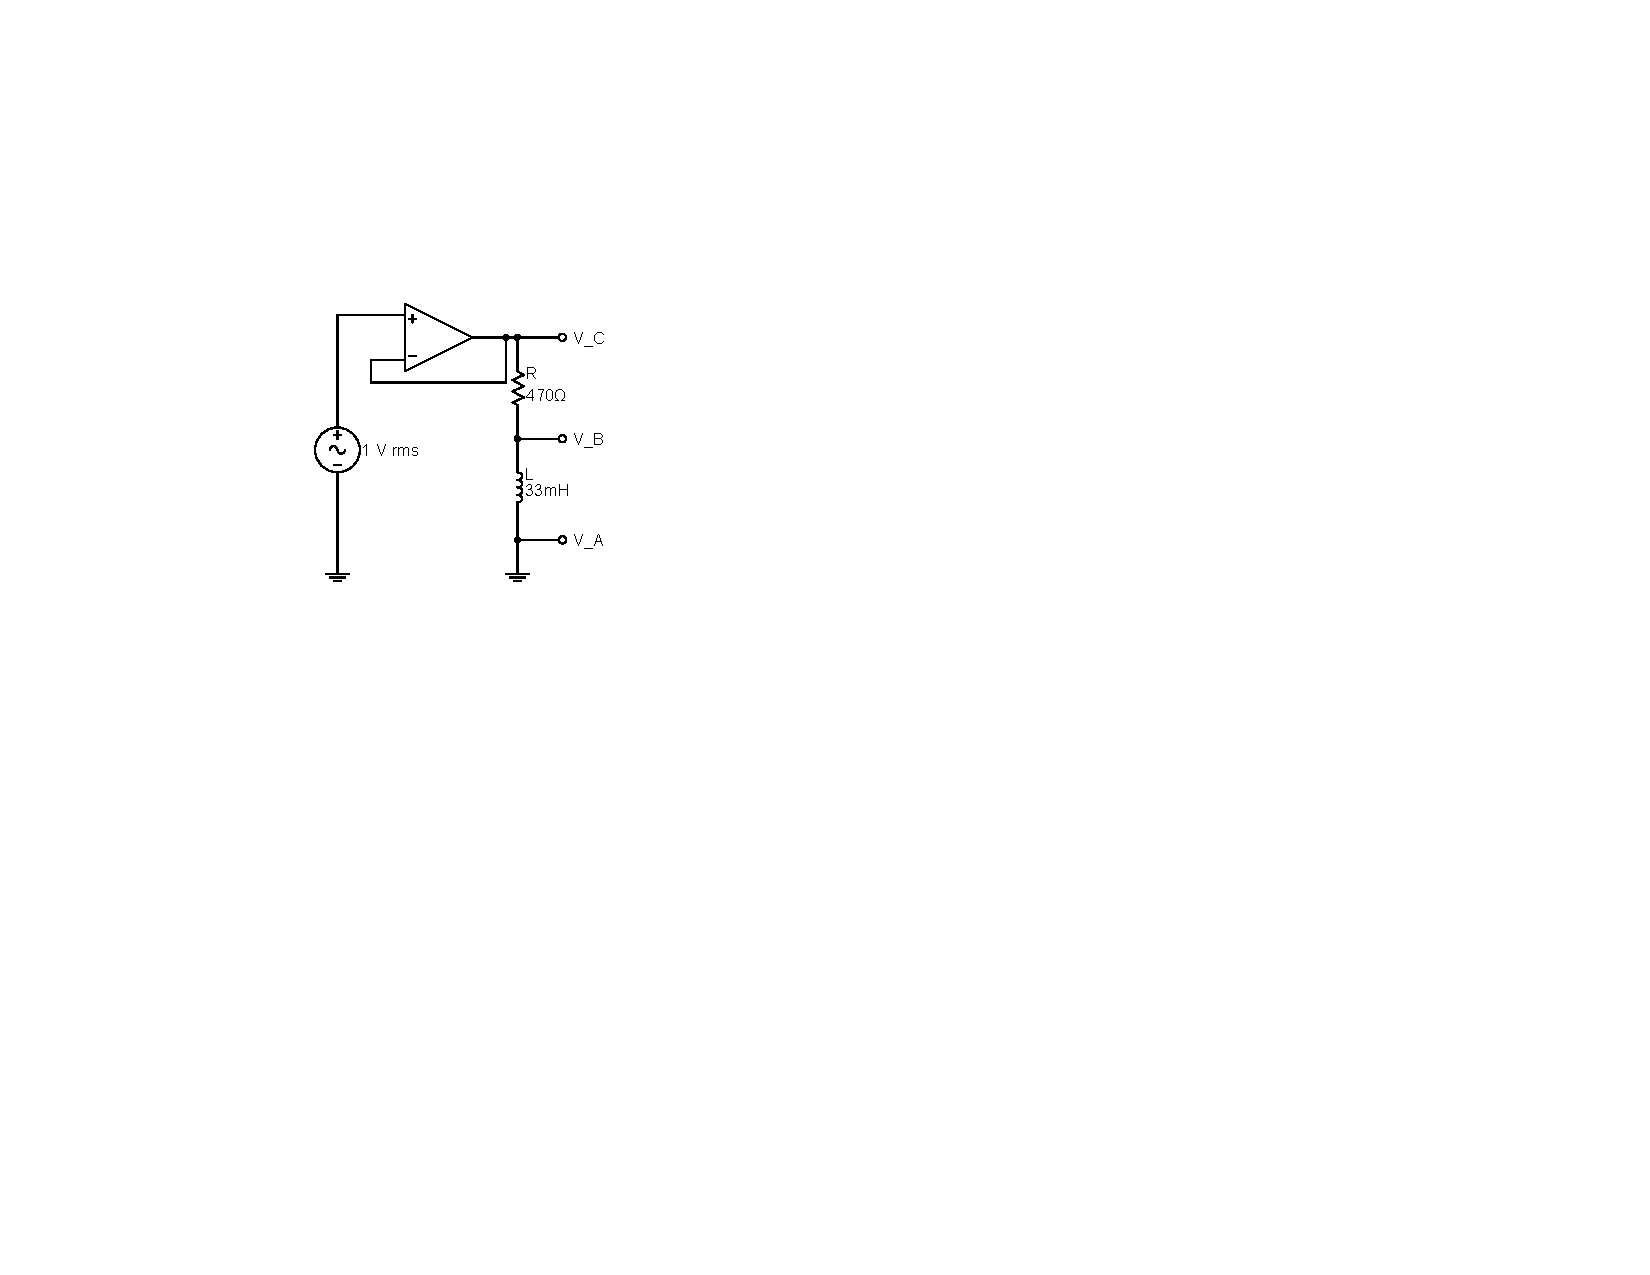
\includegraphics{ac_circuits/RandL.pdf}
\end{center}
\end{minipage}
\begin{minipage}{.4\textwidth}
\begin{center} 
\begin{tabular}{|l|c|c|} 
\hline & 20 Hz & 20 kHz \\ 
\hline $\Delta V_{BC}$ ($V_R$) & & \\ 
\hline $\Delta V_{AB}$ ($V_L$) & & \\ 
\hline $\Delta V_{AC}$ & & \\ 
\hline 
\end{tabular} 
\end{center}
\end{minipage}


\item Think of the inductor as part of a voltage divider circuit.  How does the inductor's ``resistance'' (actually its ``impedance,'' $Z_L$) depend on the angular frequency $\omega$, where $\omega = 2 \pi f$?

\item Adjust the \textit{frequency} of the generator so that the RMS value of $V_{AB}$ is about 30\% of $V_{AC}$, which should be somewhere in the neighborhood of around $f \approx 1$~kHz.  Predict what will happen to $V_{AB}$ if the 33~mH inductor is replaced by 10~mH.  Test your prediction.

\item Based on your previous answer, how does the inductor's ``resistance'' (actually its ``impedance,''  $Z_L$) depend on its inductance $L$?  Take a stab at writing a single equation relating $Z_L$ to both $\omega$ and $L$.
\label{part_guess_Z_L}

\item (Today's shocker!) With the 33~mH inductor back in place, adjust the frequency of the generator so that the RMS value of $V_{AB} = V_{BC}$, which should be around $f \approx 2$~kHz.   Is it still the case that $V_{AB} + V_{BC} = V_{AC}$?  How can this be?  Use your oscilloscope to measure all three voltages versus time, and demonstrate that Kirchoff's loop rule is not being violated here.  (Use channel 1 for $V_B$, channel 2 for $V_C$, and the difference Ch$2- $Ch1 for $V_{BC}$.)

\item Graph the voltage across the inductor and the current as a function of time.  What is the relative phase shift between them?  Does the current ``lead'' the voltage, or does the voltage ``lead'' the current? (Which one reaches its maximum value first?) \label{part_RL_graphs}

\newpage

\item Now construct the circuit below. Again, use either the DMM or your oscilloscope to measure all three RMS voltages  $V_{AB}$,  $V_{BC}$, and $V_{AC}$.   Do it for frequencies of 20~Hz and 20~kHz.\footnote{If you measure the voltages on your oscilloscope, you may notice that the waveform looks somewhat distorted at high frequencies.  If so, you can use a slightly lower frequency, say 10~kHz.  Alternatively, you can insert a 1~k$\Omega$ resistor between the output of the op-amp ($V_C$) and the +15~volt power supply, which interestingly doesn't change the level of the output, but completely eliminates the distortion!}  Is there more current in this circuit at high frequencies or low frequencies?

\begin{minipage}{.55\textwidth}
\begin{center}
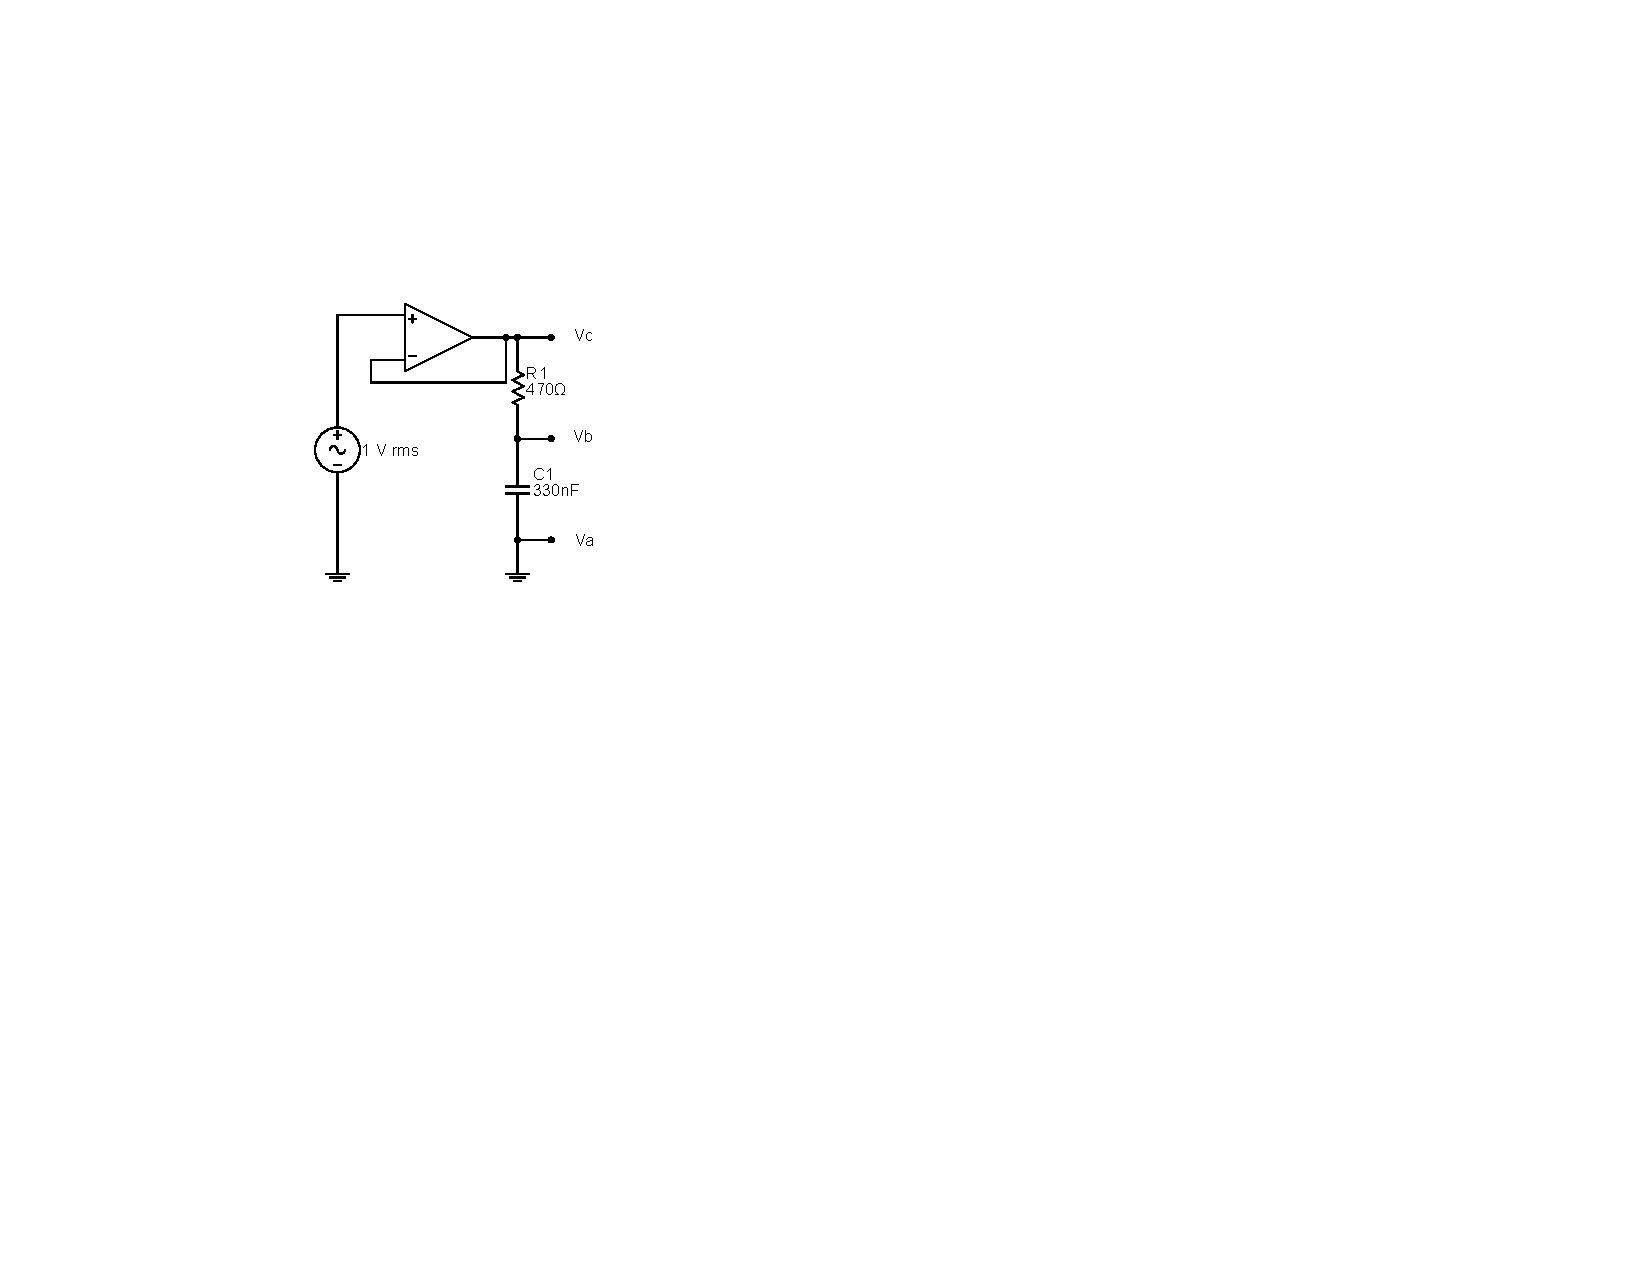
\includegraphics{ac_circuits/RandC.pdf}
\end{center}
\end{minipage}
\begin{minipage}{.4\textwidth}
\begin{center} 
\begin{tabular}{|l|c|c|} 
\hline & 20 Hz & 20 kHz \\ 
\hline $\Delta V_{BC}$ ($V_R$) & & \\ 
\hline $\Delta V_{AB}$ ($V_{cap}$) & & \\ 
\hline $\Delta V_{AC}$ & & \\ 
\hline 
\end{tabular} 
\end{center}
\end{minipage}

\item Think of the capacitor as a resistor in a voltage divider circuit: how does its ``resistance'' (actually its ``impedance,'' $Z_C$) depend on the angular frequency $\omega$, where $\omega$, where $\omega = 2 \pi f$?

\item Adjust the \textit{frequency} of the generator so that the RMS value of $V_{AB}$ is about 0.1 volts.  Predict what will happen to $V_{AB}$ if the 330~nF capacitor is replaced by 100~nF.  Test your prediction.  

\item Based on your previous answer, how does the capacitor's ``resistance'' (actually its ``impedance,'' $Z_C$) depend on its capacitance $C$?  Take a stab at writing a single equation relating $Z_C$ to both $\omega$ and $C$.
\label{part_guess_Z_C}

\item Adjust the frequency of the generator so that the RMS value of $V_{AB} = V_{BC}$.   Again, is it the case that $V_{AB} + V_{BC} = V_{AC}$?  Again, use your oscilloscope to measure all three voltages versus time, and demonstrate that Kirchoff's loop rule is not being violated here.  

\item Graph the voltage across the capacitor and the current through the capacitor as a function of time.  What is the relative phase shift between them?  Does the current ``lead'' the voltage, or does the voltage ``lead'' the current? \label{part_RC_graphs}

\vfill

\item In parts \ref{part_guess_Z_L} and \ref{part_guess_Z_C}, you probably came up with the relationships $Z_L = \omega L$ and $Z_C = 1/ \omega C$.  Those are \textit{close} to being correct, but they don't quite capture everything we want.  Ideally, we'd like for those impedances to follow something like Ohm's law, where $V_L = I Z_L$, and $V_C = I Z_C$.  But if  $I(t) = I_0 \cos(\omega t)$, do the equations $Z_L = \omega L$ and $Z_C = 1/ \omega C$ really give the correct voltages for the inductor and the capacitor?  Why not?  Think about your graphs for parts~\ref{part_RL_graphs} and \ref{part_RC_graphs}, and think carefully about whether the current and voltage are really proportional to each other in each case.

\vfill

\end{enumerate}





